\chapter{Fejlesztői dokumentáció} % Developer guide
\label{ch:impl}

\section{A NES felépítése}

\begin{figure}[H]
	\centering
	\includegraphics[scale=0.22]{mobo.jpg}
	\caption{A NES alaplapja}
\end{figure}

A NES emulációjához a következő komponenseket kell megismernünk és megvalósítanunk:

\begin{compactdesc}
	\item[Ricoh RP2A03:] 
	\hfill \\
	A hangchipet és központi feldolgozóegységet (CPU) tartalmazó integrált áramkör. Utóbbi nem más, mint az Apple II-ben és Commodore 64-ben használt 8-bites MOS Technology 6502.
	\item[Ricoh RP2C02:]
	\hfill \\
	A képfeldolgozó egység, rövid nevén PPU (Picture Processing Unit).
	\item[NROM és UNROM:] 
	\hfill \\
	Az emulátor által támogatott két kazettatípus integrált áramkörei.
	\item[Sztenderd NES kontroller:] 
	\hfill \\
	A konzol alapértelmezett beviteli eszköze.
\end{compactdesc}

\section{Órajel-frekvenciák}
A párhuzamosan működő komponenseket az órajelek hangolják össze. Az órajel-frekvencia határozza meg, hogy egy másodperc alatt hány atomi műveletet végez el egy komponens.
Minden komponens rendelkezik egy saját órajelfrekvenciával, amit egy központi órajelből származtatnak.

\begin{itemize}
	\item Központi órajel-frekvencia: $ f = \frac{236.25\;MHz}{11} \sim 21.477272\; MHz $
	\item CPU órajel-frekvencia: $ \frac{f}{12} \sim 1.789773 \; MHz  $
	\item PPU órajel-frekvencia: $ \frac{f}{4}  \sim 5.369318 \; MHz $
\end{itemize}

\section{A központi feldolgozóegységhez kapcsolódó fogalmak}

\begin{note}
	A hexadecimális értékeket \textbf{\$} prefix-el jelölöm.
\end{note}

\subsection{Opkód} 
Egy opkód a 6502 esetében csupán egyetlen bájt, amiből az utasításdekódoló egyértelműen meg tudja határozni a végrehajtandó utasítást és annak címzési módját.
Ezt a hozzárendelést az opkódmátrix írja le. Az emulációhoz emellett azt is tárolni kell az opkódmátrixban, hogy a végrehajtandó művelet hány központi órajel alatt fejeződik be, ugyanis csak ennek ismeretében tudjuk a CPU-t és a PPU-t precízen egymáshoz szinkronizálni.

\begin{figure}[H]
	\centering
	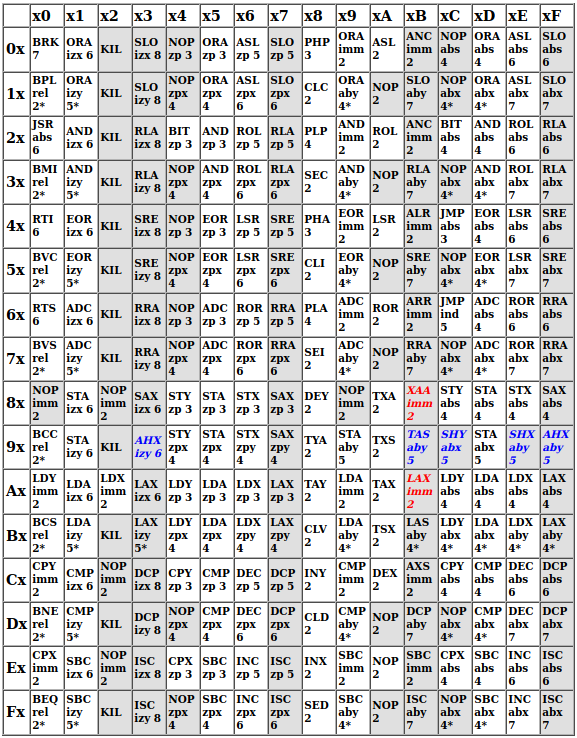
\includegraphics[scale=0.65]{opcodes.png}
	\caption{A 6502 opkódmátrixa}
	\label{fig:opcodes}
\end{figure}

Ha meg szeretnénk találni egy adott opkódhoz a hozzá tartozó információt, akkor szükségünk lesz az opkód hexadecimális alakjára, ami legfeljebb kétszámjegyű lehet. A nagyobb helyiértékű számjegy a keresett cella sorát, a kisebbik pedig az oszlopát írja le. Példaként a \ref{fig:opcodes} ábrán láthatjuk, hogy a \textbf{\$30} opkódhoz a BMI utasítás tartozik relatív címzéssel.
Azok az opkódok csillaggal vannak jelölve, amiknek a futási ideje megnőhet az aktuális argumentumoktól függően.
A szürkével jelölt opkódokhoz hivatalosan nincs utasítás rendelve. 
Ezeket a nem dokumentált, ``illegális'' opkódokat a processzor későbbi 
verzióinak hagyták fent. A tervezők nem tiltották meg azonban ezeknek a használatát, 
egyszerűen csak nem definiálták a viselkedésüket. Ennek ellenére több olyan illegális opkód is belekerült a dizájnba, ami később hasznosnak bizonyult. A játékfejlesztők próbálkozások útján
felfedezték, hogy melyek azok az opkódok, amiknek a viselkedése determinisztikus és néhány speciális feladat esetén érdemes őket használni.
Ritka ugyan, de van olyan játék, ami ezeket az opkódokat is használja, ezért ezeknek az opkódoknak az emulációját is megvalósítottam.

\subsection{Regiszterek}
A regiszter a processzor leggyorsabban elérhető memóriája.
A gyártási költségek alacsonyan tartása végett csak 6 regiszter került a processzorba.
Minden regiszter mellett zárójelben fel van tüntetve annak mérete bitekben megadva.

\begin{compactdesc}
	\item[A (8):] Akkumulátor, az aritmetikai műveletek eredményei ebbe kerülnek.
	\item[X (8) és Y (8):] 
	Index regiszterek, indirekt címzésnél használjuk őket.
	Ciklusok esetén a ciklusváltozót érdemes ezekben tárolnunk.
	\item[S (8):] 
	Verem mutató. A verem tetejének a kezdőcímtől vett eltolását tárolja.
	\item[P (8):]
	Státusz regiszter, ami 7 darab flag bitet tárol.
	\item[PC (16):]
	Programszámláló. 
	A következő opkód memóriacímét tárolja.
	Méretéből következik, hogy a processzor teljes címtartománya 64 KiB nagyságú.
\end{compactdesc}


\subsection{Memórialap}
Az $i$. lap egy 256 bájtos egybefüggő memóriarész, ami a $ [i \cdot \$100, \: (i+1) \cdot \$100) $ címtartományon helyezkedik el.

\subsection{Hívási verem}
Az egymásba ágyazott eljárásokat a processzor hardveresen támogatja, amihez egy vermet használ.
A verem az 1. lapon található, és a kisebb címek felé nő.
Eljárás hívásakor a verem tetejére kerül az aktuális programszámláló értéke, 
visszatéréskor pedig a veremről levett címre állítjuk be a programszámláló értékét.

\subsection{Megszakítás}
A komponensek kommunikációjának egyik módja a hardveres megszakítás.
A 6502 chip egy darab maszkolható \emph{(IRQ)} és egy nem maszkolható \emph{(NMI)} megszakítási lábbal rendelkezik.
A megszakítási vektorokkal a program beállíthatja, hogy egy bizonyos megszakításra milyen szubrutinnal kíván reagálni. A vektorok 2 bájtos tárolók, amik a kezelő szubrutin címét tartalmazzák. Az NMI-hez tartozó vektor a \$FFFA és a \$FFFB címeken, míg az IRQ-hoz tarozó vektor az \$FFFE és a \$FFFF címeken található. A 6502 ``kicsi az elején'' bájtsorrendű (little-endian) processzor, ezért a címeknek mindig az alsó 8 bitjét tárolja az alacsonyabb címen, a felső 8 bitjét pedig a magasabb címen.
A program dönthet úgy, hogy a maszkolható megszakítást figyelmen kívül hagyja (a kezelő szubrutin nem hívódik meg), ehhez az \emph{IRQ Disable} flag-et be kell állítania a státusz regiszterben. A nem maszkolható megszakítás esetén erre nincsen lehetőség, a végrehajtás mindenképpen a kezelő szubrutinhoz ugrik.
A nem maszkolható lábhoz a képfeldolgozó, a maszkolhatóhoz a hangchip van kötve.

\subsection{Opkód argumentum helye, fajtája}

\begin{figure}[H]
	\centering
	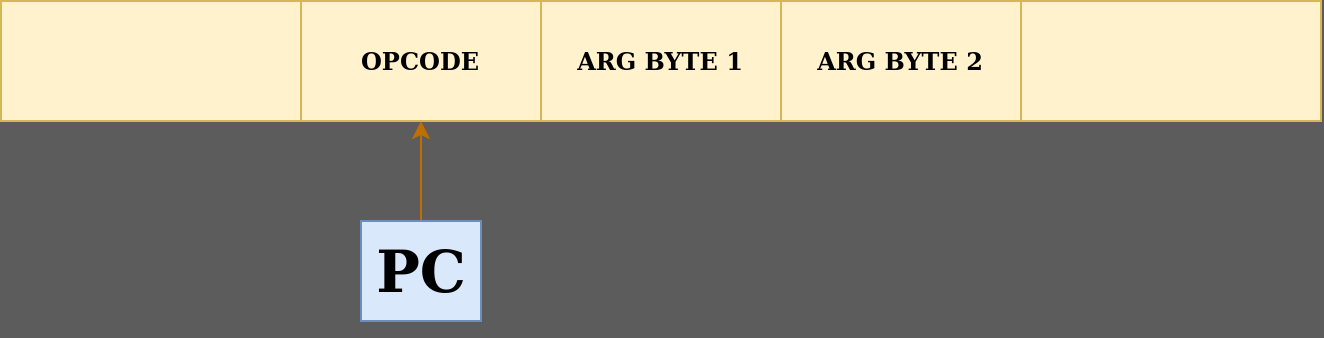
\includegraphics[scale=0.25]{opcode.png}
	\caption{Opkód argumentumainak helye}
	\label{fig:argplacement}
\end{figure}

A \ref{fig:argplacement} ábra szemlélteti, hogy az opkód argumentumok közvetlenül az opkód mögött, a \emph{PC+1} és \emph{PC+2} címeken helyezkedhetnek el a memóriában. Címzési módtól függően változhat az argumentumok száma 0, 1 és 2 bájt között.
Ha az opkód rendelkezik argumentummal vagy argumentumokkal, akkor azok a következő fajtájúak lehetnek:

\begin{compactitem}
	\item 2 bájt, ami abszolút memóriacímet ábrázol kicsi-az-elején bájtsorrenddel 
	\item 1 bájt, ami relatív eltolást ír le
	\item 1 bájt, ami a művelet közvetlen operandusa
\end{compactitem}

\subsection{Címzési módok}

Egy opkód után azoknál a címzési módoknál áll argumentum, amiknél a művelet elvégzéséhez 
szükséges operandus nem regiszterben, hanem a memóriában van. A címzési módok azt határozzák meg, hogy az argumentumból hogyan kell kiszámolni az operandus effektív 16 bites memóriacímét. Az alábbiakban felsorolt  címzési módoknál a zárójelben az opkódmátrixbeli név (amennyiben van) és az argumentum bájtok száma található.  


\begin{description}
	\item[Akkumulátor mód (0):] nincs argumentum, az utasítás az \textbf{A} regiszter értékét módosítja.
	\item[Azonnali mód (imm, 1):] az utasítás operandusa maga az argumentum. Jele: \#
	\newline
	Példa: az LDA \#\$0 utasítás nullára állítja az \textbf{A} regisztert.
	\item[Abszolút mód (abs, 2):] az argumentum az operandus effektív címe.
	\item[0. lap mód (zp, 1):] A CPU kevés regiszterét azzal ellensúlyozták, hogy ennek a speciális módnak köszönhetően a nulladik lapot hatékonyabban lehet címezni, mint a többit. 
	Mivel a 0. lap mérete 256 bájt, ezért teljes cím helyett elég egyetlen bájt a címzéséhez.
	A kisebb paraméter gyorsabban beolvasható és egyúttal a kódméretet is csökkenti.
	\item[Indexelt 0. lap mód (zpx, zpy, 1):]
	Hasonlóan most is csak a 0. lapot tudjuk címezni, de az argumentumhoz hozzáadjuk valamelyik index regiszter értékét.
	Az operandus címének kiszámítása: $ (arg1 + index) \mod 256 $
	\item[Indexelt abszolút mód (abx, aby, 2):] Az argumentumok egy teljes memóriacímet alkotnak, amihez hozzáadjuk a megadott index regiszter értékét. 
	\item[Implicit mód (0):] nincs szükség argumentumra, mert az utasítás regiszterekkel dolgozik.
	\item[Relatív mód (rel, 1):] Az elágazási utasítások használják ezt a címzési módot. Elágazásoknál ha a feltétel teljesül, akkor az argumentummal el kell tolni a programszámlálót. Az elágazási utasítások feltételeit lásd az \emph{\nameref{instructionset}} szekcióban.
	\item[Indirekt mód (ind, 2):] 
	Erre a címzési módra a JMP utasításnál van szükség.
	A két argumentum bájt együtt egy teljes memóriacímet alkot, legyen ez \emph{m}.
	Az operandus címét az \emph{m} és \emph{m+1} címeken találjuk, így tehát az operandus értékét a következő módon kapjuk meg: $$ operand := read(\;(read(m+1) << 8) \;\; | \;\; read(m)\;) $$
	\item[Indexelt indirekt mód (izx, 1):]
	Az X regisztert összeadjuk az argumentummal, így egy 0. lapon található címet kapunk.
	Erről a címről kell az operandus effektív címét kiolvasni.
	\begin{figure}[H]
		\centering
		\vspace{0.4cm}
		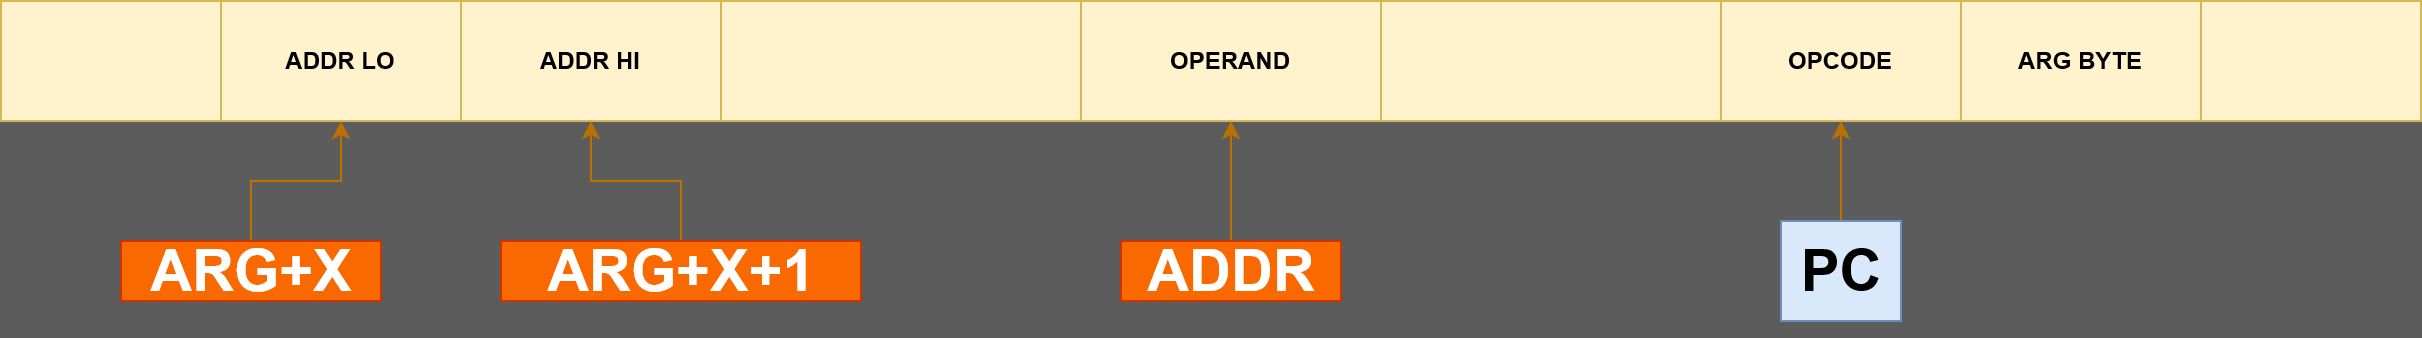
\includegraphics[width=1.1\textwidth,height=70px]{indexed_indirect.png}
		\caption{Indexelt indirekt címzés}
	\end{figure}
	\item[Indirekt indexelt mód (izy, 1):]
	Az argumentum egy 0. lapon található címre mutat, amit ha összeadunk az Y regiszter értékével, akkor megkapjuk az operandus effektív címét. 
	
	
	
\end{description}

Az \textbf{abx}, \textbf{aby} és \textbf{izy} indexelt címzési módok és bizonyos utasítások kombinációjánál előfordulhat, hogy a végleges operandus cím és az indexelés előtt álló cím különböző memórialapra esik. Ebben az esetben 1 órajelciklussal tovább tart az utasítás végrehajtása.
Emellett az elágazási utasítások (relatív címzés) több ciklus alatt fejeződnek be, ha az ugrási feltétel teljesül. Ha az ugrás előtti PC értéke és az ugrási cél más lapra esik, akkor +2, ellenkező esetben csak +1 órajelciklussal kell számolni.

\subsection{Memóriatérkép}

A memóriatérkép leírja a címtér felosztását a komponensek között.
A memóriatérképből meg tudjuk állapítani, hogy egy adott címen található bájt kiolvasásához vagy írásához melyik komponens hardveres logikáját kell alkalmazni.

\begin{table}[H]
	\centering
	\begin{tabular}{ | l | l | }
		\hline
		Tartomány & Eszköz \\
		\hline			
		$ \$0000 - \$07FF $ & CPU RAM \\
		$ \$0800 - \$1FFF $ & CPU RAM tükrözése \\
		$ \$2000 - \$2007 $ & PPU regiszterek \\
		$ \$2008 - \$3FFF $ & PPU regiszterek tükrözése \\
		$ \$4000 - \$4017 $ & APU és IO regiszterek \\
		$ \$4018 - \$401F $ & APU és IO regiszterek tükrözése \\
		$ \$4020 - \$FFFF $ & Kazetta \\
		\hline
	\end{tabular}
\end{table}

\subsection{Memóriatükrözés}
Memóriatükrözésről beszélünk, amikor fizikailag ugyanazt a memóriaterületet több memóriacímről is el tudjuk érni. Ha egy címtartomány $x$ bájtonként tükrözve van, akkor minden olyan $a$ és $b$ memóriacím ugyanarra a bájtra mutat, ami a tartományba vagy a tükrözésébe esik és $a \equiv b\ (\textrm{mod}\ x)$.  A CPU RAM 2 KiB-onként tükrözve van, amiből következik, hogy a \textbf{\$0001}, \textbf{\$0801} \textbf{\$1001}, \textbf{\$1801} címek ugyanarra a bájtra mutatnak. Egy címtartomány tükrözése lehet nagyobb mint az eredeti tartomány (például a CPU RAM esetében a tükrözési tartomány háromszor nagyobb).

\subsection{Státusz flagek}

\begin{compactenum}
	\setcounter{enumi}{-1}
	\item bit: C = Carry \newline Összeadások, forgatások, eltolások során a leeső biteket jelzésére.
	\item bit: Z = Zero   \newline Aritmetikai művelet eredménye vagy mozgatott bájt 0.
	\item bit: I = IRQ Disable
	\newline Az 1-re állításával maszkoljuk az IRQ-t.
	\item bit: D = Decimal mode
	\newline
	A NES nem használja ezt a flag-et.
	\item bit: B = BRK Command
	\newline Az 1-re állításával generálhatunk egy szoftveres megszakítást. 
	\setcounter{enumi}{5}
	\item bit: V = Overflow
	\newline 
	Aritmetikai műveleteknél a túlcsordulás vagy alulcsordulás jelzésére.
	A BIT utasítás speciálisan használja.
	\item bit: N = Negative
	\newline A manipulált bájt negatív, vagyis a legnagyobb helyiértékű bitje 1.
\end{compactenum}

\subsection{Utasításkészlet}
\label{instructionset}

\begin{compactdesc}
	\item Aritmetikai és logikai egység (ALU)
	\begin{compactdesc}
		\item[ADC:] Összeadás
		\item[SBC:] Kivonás
		\item[AND:] Logikai ÉS művelet
		\item[ASL:] Bájt balra elcsúsztatása
		\item[LSR:] Bájt jobbra elcsúsztatása
		\item[ORA:] Logikai VAGY
		\item[EOR:] Kizárásos VAGY
		\item[INC, INX, INY:] növelés eggyel
		\item[DEC, DEX, DEY:] csökkentés eggyel
		\item[ROL, ROR:] bájt forgatása
	\end{compactdesc}
	\item 
	Összehasonlítás, tesztelés
	\begin{compactdesc}
		\item[CMP, CPX, CPY:]  \hfill \\ A megadott címen található bájt és rendre az A, X és Y regiszterekben található bájt között az $=$ és a $>=$ reláció kiértékelése
		\item[BIT:] Az operandus bájt maszkolása (\&) az A regiszter tartalmával, az eredmény szerint a Z,N,V flag-ek frissítése 
	\end{compactdesc}
	\item Veremműveletek
	\begin{compactdesc}
		\item[PHA:] Az akkumulátor regiszter értékének felrakása a veremre 
		\item[PHP:] A státusz regiszter értékének felrakása a veremre
		\item[PHA:] Az akkumulátor regiszter új értékének levétele a veremről
		\item[PHP:] A státusz regiszter új értékének levétele a veremről
	\end{compactdesc}
	\item Vezérlés
	\begin{compactdesc}
		\item[JMP:] Vezérlés áthelyezése egy megadott memóriacímhez, avagy a programszámláló átállítása erre a címre
		\item[JSR:] Szubrutin hívás (visszatérési cím elmentése + \textbf{JMP})
		\item[RTS:] Visszatérés szubrutinból (visszatérési cím kiolvasása + \textbf{JMP})
		\item[BRK:] Szoftveresen generált megszakítás
		\item[RTI:] Visszatérés megszakításkezelőből
	\end{compactdesc}
	\item Flag manipuláció (a utasításnév harmadik betűje a változtatott flag-et jelöli) \newline \textbf{CLC, CLD, CLI, CLV, SED, SEC, SEI}
	\newline
	(C = Clear, S = Set)
	\item Elágazások: vezérlés áthelyezése akkor, ha teljesül a feltétel az utasítás által vizsgált státusz flag-re
	\newline \textbf{BCC(C=0), BCS(C=1), BNE(Z=0), BEQ(Z=1), BPL(N=0), BMI(N=1),  BVC(V=0), BVS(V=1)}
	\item Bájtok mozgatása regiszterek és a memória között
	\newline
	\textbf{LDA, LDX, LDY, STA, STX, STY} 
	\newline
	(L = Load, S = Store)
	\newline
	A név harmadik betűje a használt regisztert jelöli.
	\item Bájtok mozgatása regiszterek között
	\newline
	\textbf{TAX, TAY, TSX, TXA, TXS, TYA}
	\newline
	A név második betűje a forrásregisztert, a harmadik a célregisztert jelöli.
\end{compactdesc}

\section{Kazetták}

A kazettákon logikai szempontból kétfajta memória található: PRG és CHR.
A PRG jellemzően csak olvasható memória (ROM), ahol a processzor által végrehajtandó utasítások, avagy a játéklogika kapott helyett. Mérete NROM esetében 16 KiB vagy 32 KiB, UNROM-nál pedig 64 KiB vagy 128 KiB. A 8 KiB méretű A CHR ROM/RAM memória, mely 8 KiB méretű és játék sprite-jait tárolja, amik 8*8 pixeles kis képekből állnak. Ezeket a kis képeket ezentúl alakzatoknak fogom hívni. 

\subsection{Az iNES fájlformátum}

Az iNES fájlformátumot egy korai NES emulátor vezette be a NES játékok bináris formában történő terjesztésére. A fájl elején található 16 bájtos fejléc többek között a mapper áramkör azonosítóját, a képfeldolgozó névtábláinak tükrözési módját, valamint a PRG ROM és a CHR memóriák típusát (ROM/RAM) és méretét határozza meg. A fejléc után ezek tartalma található.

\section{A képfeldolgozó egység}

\subsection{Színpaletta}

A képpontok végső RGB színkódjának meghatározása többféle módon is lehetséges. A gyors, de kevésbé pontos módszer, ha egy fix palettával dolgozunk. A paletta hozzárendel egy $\$0$ és $\$3F$ közötti azonosítóhoz egy színkódot, így tehát 55 különböző színt tudunk megjeleníteni. A lassabb, de pontosabb módszer, hogy az analóg NTSC videójelre történő konverziót is emuláljuk. Az emulátoromnál a gyorsabb módszert implementáltam.

\vspace{0.3cm}
\begin{figure}[H]
	\centering
	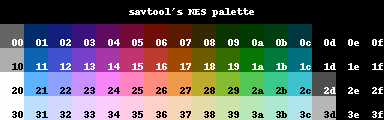
\includegraphics{palette.png}
	\caption{A 2C02 színpalettája}
\end{figure}

\clearpage

\subsection{Paletta indexek}

A $\$3F00 - \$3F1F$ címtartományon található paletta indexben kerülnek eltárolásra a használatban lévő színek színpalettabeli azonosítói, csoportokba (palettákba) rendezve. A hardveres limitációk miatt a hátteret 16x16 pixeles cellákra osztották fel. Egy cellán belül kizárólag 4 féle szín fordulhatott elő. Ezeket a 4 színből álló színkombinációkat kissé megtévesztő módon szintén palettáknak nevezik. További limitáció, hogy a paletták 4. színe nem változtatható, mert ezek mindig a \$3F00 címet (a háttérszínt) tükrözik.

\begin{table}[H]
	\centering
	\begin{tabular}{ | l | l | }
		\hline
		Tartomány & Paletta \\
		\hline			
		$ \$3F00 $ & Univerzális háttérszín \\
		$ \$3F01 - \$3F03 $ & 0. háttér paletta \\
		$ \$3F05 - \$3F07 $ & 1. háttér paletta \\
		$ \$3F09 - \$3F0B $ & 2. háttér paletta \\
		$ \$3F0D - \$3F0F $ & 3. háttér paletta \\
		$ \$3F11 - \$3F13 $ & 0. sprite paletta \\
		$ \$3F15 - \$3F17 $ & 1. sprite paletta \\
		$ \$3F19 - \$3F1B $ & 2. sprite paletta \\
		$ \$3F1D - \$3F1F $ & 3. sprite paletta \\
		\hline
	\end{tabular}
	\caption{A paletta RAM struktúrája}
	\label{fig:paletteram}
\end{table}

\subsection{Alakzattáblázat}

A CHR memóriában található két alakzattáblázat az alakzatokat tárolja egy speciális formátumban. Ha az alakzatokat úgy reprezentálnánk, hogy minden pixelre eltárolnánk egy színkódot, akkor pixelenként 6 bitre lenne szükségünk (mivel 55 színkódból választhatunk). Ehelyett pixelenként csak 2 bitet (egy szignifikáns és egy kevésbé szignifikáns bitet) tárolnunk, amik együtt egy, a palettaindexben található palettán belüli színt azonosítanak. Az attribútumtábla segítségével fogjuk később meghatározni, hogy a vizsgált pixelhez melyik paletta tartozik. Mivel a paletta index írható és olvasható memória is, így a program futási időben, dinamikusan változtathatja, hogy egy paletta milyen színeket tartalmaz, ezáltal pár lépésben átszínezheti az összes alakzatot, ami az adott palettát használja.
Egy alakzattáblázat 16x16 darab alakzatot tartalmaz és egy alakzat 8x8 pixeles, ebből adódóan a táblázat teljes mérete $16\cdot16\cdot(8\cdot8\cdot2)\div8 = 4096$ bájt. Egy alakzat pixeljeinek bitjeit $(8\cdot8\cdot2)\div8 = 16$ egymást követő bájt tárolja a \ref{fig:patt} ábrán szemléltetett módon. Először 8 bájton keresztül a kevésbé szignifikáns bitek, majd ezután újabb 8 bájton át a szignifikánsabb bitek helyezkednek el.

\begin{figure}[H]
	\centering
	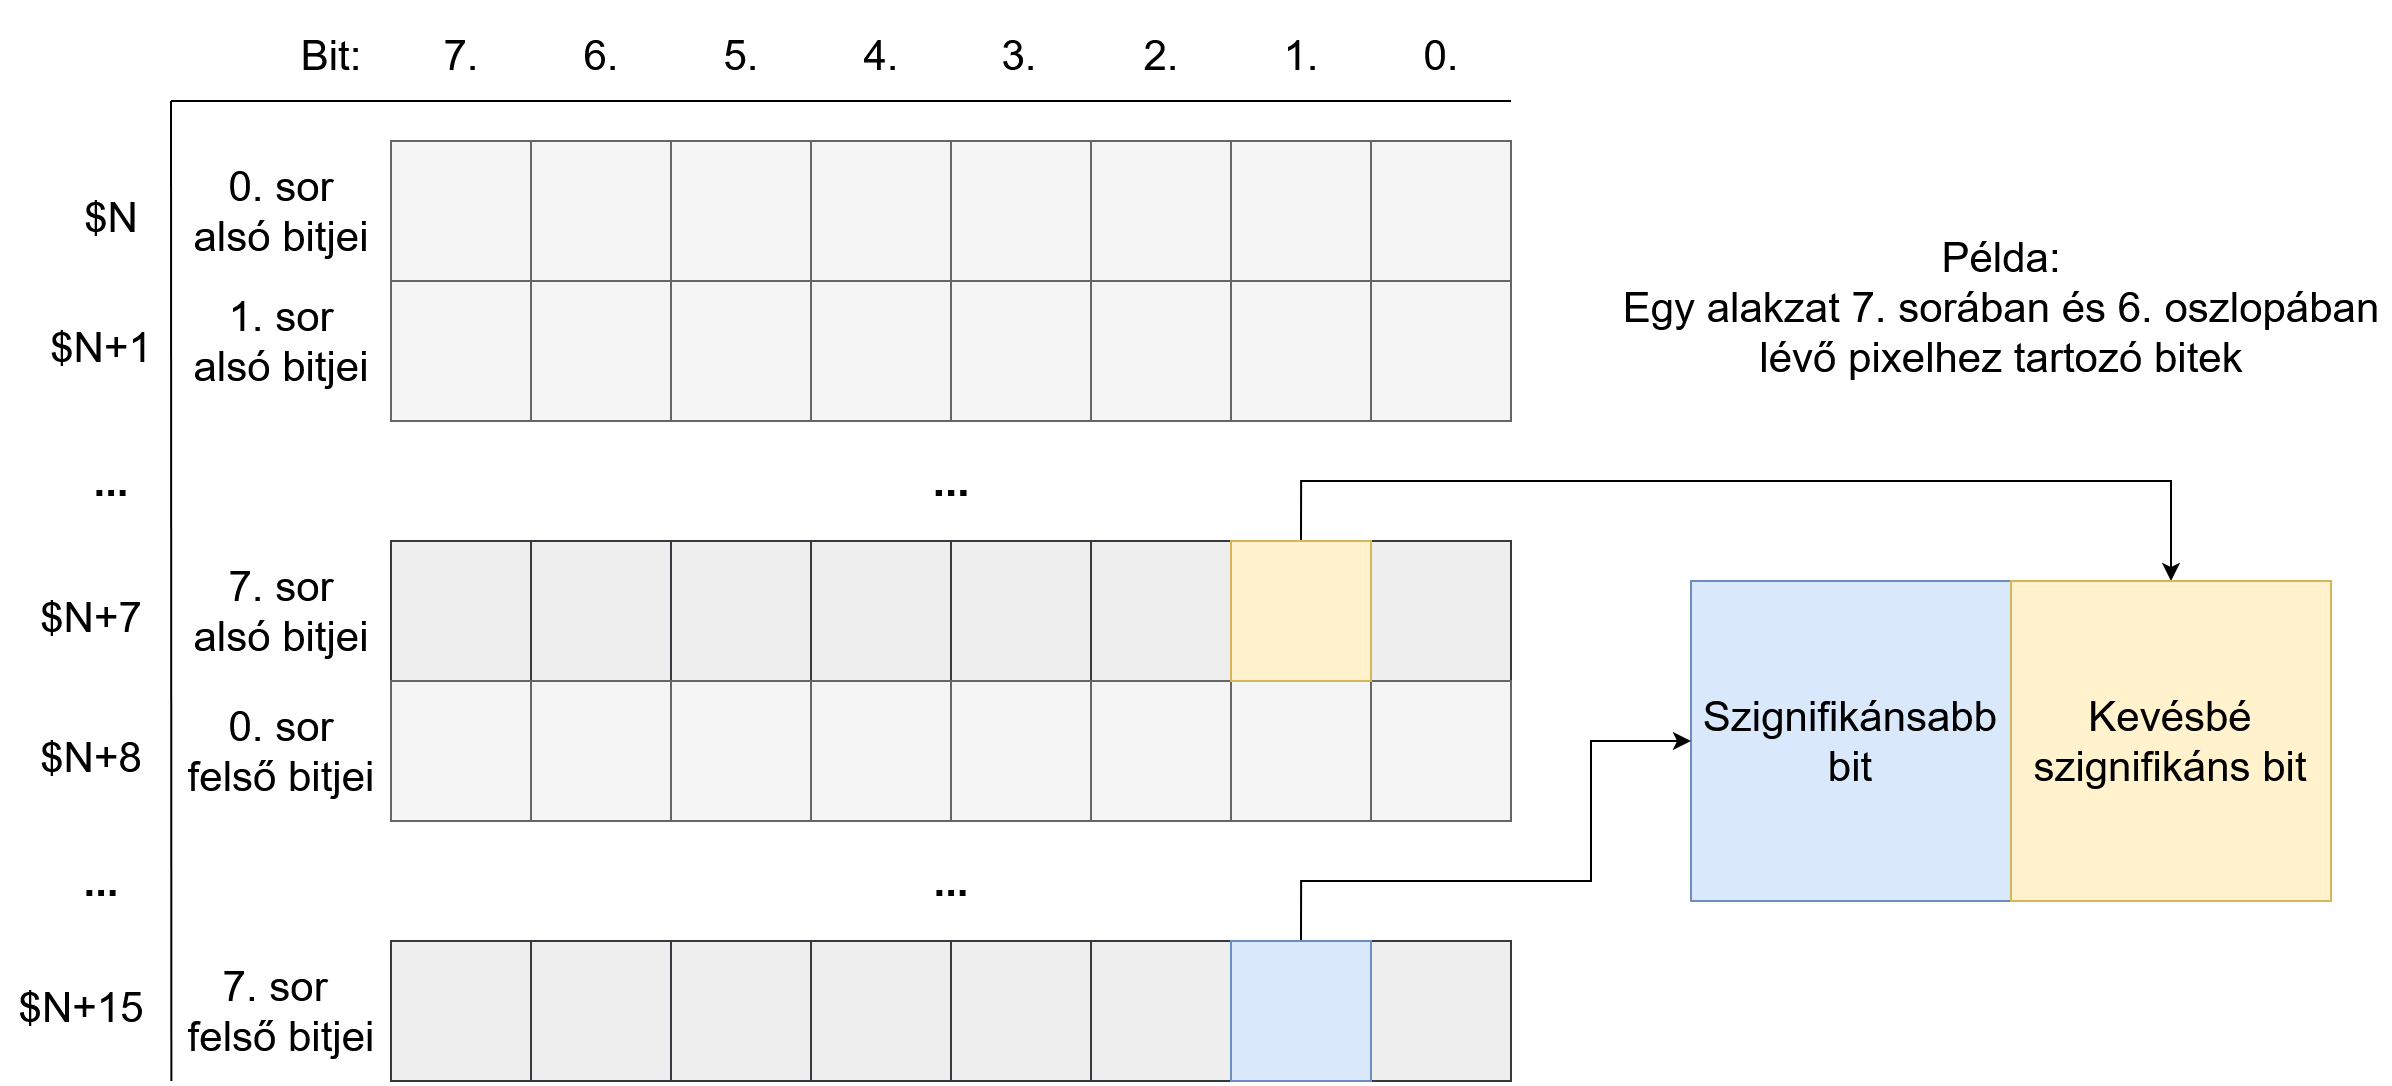
\includegraphics[scale=0.175,frame]{patt.png}
	\caption{Egy alakzat reprezentálása}
	\label{fig:patt}
\end{figure}


\begin{figure}[H]
	\centering
	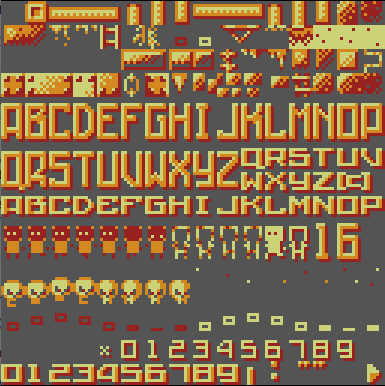
\includegraphics[width=0.45\linewidth,frame]{patt2.png}
	\hspace{5pt}
	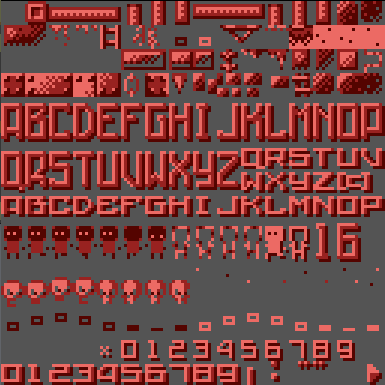
\includegraphics[width=0.45\linewidth,frame]{patt1.png}
	\caption{Az Alter Ego játék 0. alakzattáblázata különböző palettákkal kirajzolva}
\end{figure}

\subsection{Rétegek}
A képfeldolgozó két réteget képes kezelni hardveresen, ezek a háttér és a sprite rétegek.
Általában a képkocka azon részei tartoznak a háttérhez, amik ritkán változnak (például feliratok, számlálók, mozdulatlan képek) és a kirajzolásukhoz nem szükséges további transzformáció (eltolás, tükrözés). A háttérben az alakzatok 30 sorból és 32 oszlopból álló négyzetrácsot alkotnak (ebből és az alakzatok méretéből ered a NES 256*240 pixeles felbontása).
A háttér rétegben egyesével nem lehet alakzatokat eltolni, csak az egész háttér eltolása lehetséges. A sprite rétegben nagyobb flexibilitás áll rendelkezésre, ugyanis itt egyenként, pixel pontosságú eltolással, valamint horizontális és/vagy vertikális tükrözéssel rajzolhatjuk ki az alakzatokat. A sprite rétegnél legfeljebb 64 alakzat szerepelhet egy képkockán (ez a megkötés a később ismertetett OAM méretéből adódik).  

\subsection{Névtáblázat}

A háttérréteg négyzetrácsának elrendezését a névtáblázatok tárolják. A névtáblázat a háttér 960 darab alakzatcellájának mindegyikéhez eltárolja a cellába rajzolandó alakzat sorszámát. Ez a sorszám relatív, ugyanis mindig azon az alakzattáblázaton belül értendő, amit a CONTROLLER regiszterrel a program kiválasztott.

\subsection{Attribútum táblák}

Minden névtáblához tartozik egy 64 bájtos attribútumtáblázat, ahol minden bájt egy 4*4 alakzatcellából álló terület palettáit határozza meg. A bájtok 4 darab 2 bites részre vannak felosztva, ahol mindegyik rész egy 2*2 cellából álló terület palettájának sorszámát (0-3) kódolja el. Ennek a reprezentációnak a következménye, hogy a háttér 4 cellából álló csoportjai mindig egy palettán osztoznak.

A 16 cellát lefedő bájt a következőképpen van felosztva a 4 cellás területek között:

\begin{figure}[H]
	\centering
	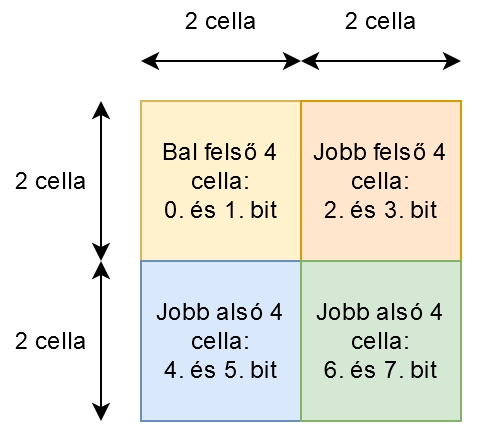
\includegraphics[width=0.4\linewidth]{attrtable.png}
\end{figure}


\subsection{Háttéreltolás}

A háttéreltolással pixelpontossággal megszabhatjuk, hogy a háttér mely része legyen látható a játékos számára.
Az eltolás miatt van szükség több névtáblára, ugyanis a lecsúszó háttérrész a valamelyik másik névtáblából lesz kiolvasva. 

\subsection{OAM (Object Attribute Memory)}

A sprite réteg elrendezését leíró 256 bájtos memória. 64 darab alakzatról tárol információt, amik a következők:

\begin{compactitem}
	\item X és Y koordináta
	\item A sprite réteg aktív alakzattáblázatán belüli sorszám
	\item Tükrözés
	\item Paletta sorszám
	\item Prioritás a háttérrel szemben
\end{compactitem}

\subsection{Regiszterek}

A CPU és a PPU az alább látható 9 darab egy bájtos regiszter segítségével tud egymással kommunikálni. A regisztereket a CPU a zárójelekben található címeken tudja elérni.
Az olvasató regiszterek \textbf{R}, az írhatók \textbf{W} betűvel vannak megjelölve.

\vspace{0.25cm}

\begin{description}
	\item[CONTROLLER(\$2000, W):] \hfill \\
	A kirajzolás vezérlésére szolgáló regiszter.
	Beállítható vele a következő képkockánál használandó táblázatok indexe.
	\begin{compactdesc}
		\item[0-1. bit:] Aktív névtáblázat indexe
		\item[2. bit:] VRAM cím inkrementálási mód
		\item[3. bit:] Aktív alakzattáblázat indexe a sprite rétegnél
		\item[4. bit:] Aktív alakzattáblázat indexe a háttér rétegnél
		\item[5. bit:] Sprite méret (8x8 vagy 8x16 pixel)
		\item[6. bit:] Az emuláció során nem használt bit
		\item[7. bit:] NMI generálása a PPU tétlen periódusának kezdetén
	\end{compactdesc}
	\item[MASK(\$2001, W):] \hfill \\
	A rétegek egyenkénti ki/bekapcsolása és speciális effektusok 
	(például szürkeárnyalat) vezérelhetők vele.
	\item[STATUS(\$2002, R):] \hfill \\
	A kirajzolás alatt bekövetkező eseményeket jelzi a PPU a CPU-nak ezzel a regiszeterrel.
	Ilyen esemény például a sprite túlcsordulás, ami akkor áll fent, ha több mint a 8 alakzat kerülne egy sorra a sprite rétegben. 
	\item[OAMADDR(\$2003, W) és OAMDATA(\$2004, R/W):] \hfill \\
	A processzor ezen két regiszter segítségével képes új adatokkal feltölteni az OAM memóriát.
	Az alábbi kódrészlet azt szemlélteti, hogy az \emph{adatok} tömb tartalmát hogyan kell a CPU memóriájából
	az OAM-ba átmásolni egy megadott címtől kezdve. Az OAMDATA írása után az OAMADDR automatikusan inkrementálódik a másolás gyorsításának érdekében.
	\begin{lstlisting}
	OAMADDR := 8 bites OAM cim
	for i in 1..adatok.hossz
		OAMDATA := adatok[i]
	\end{lstlisting}
	\item[PPUSCROLL(\$2005, W):] \hfill \\
	Beállíthatjuk vele, hogy a hátteret hány pixellel szeretnénk arrébbcsúsztatni (Horizontális tükrözésnél vízszintesen, vertikális tükrözésnél függőlegesen).
	\item[PPUADDR(\$2006, W) és PPUDATA(\$2007, R/W):] \hfill \\
	A névtáblák frissítésére szolgálnak. Hasonlóan kell őket használni, mint az OAMADDR és OAMDATA regisztereket.
	\item[OAMDMA(\$4014, W):] \hfill \\
	Az OAM memória frissítésének egy alternatív, gyorsabb módja a Direct Memory Access (DMA). Ekkor a processzorban található dedikált hardver másolja át az adatokat egyenesen a CPU RAM-ból az OAM memóriába. A másolás megkezdéséhez annak a memórialapnak a sorszámát kell beírni a regiszterbe, ahol az átmásolandó adatok találhatók.
\end{description}

\subsection{Memóriatérkép}

\begin{table}[H]
	\centering
	\begin{tabular}{ | l | l | }
		\hline
		Tartomány & Paletta \\
		\hline			
		$ \$0000 - \$0FFF $ & 0. Alakzattáblázat \\
		$ \$1000 - \$1FFF $ & 1. Alakzattáblázat \\
		$ \$2000 - \$23FF $ & 0. Névtáblázat \\
		$ \$2400 - \$27FF $ & 1. Névtáblázat \\
		$ \$2800 - \$2BFF $ & 2. Névtáblázat \\
		$ \$2C00 - \$2FFF $ & 3. Névtáblázat \\
		$ \$3000 - \$3EFF $ & A 0-3. névtáblázatok tükrözése \\
		$ \$3F00 - \$3F1F $ & Paletta indexek \\
		$ \$3F20 - \$3FFF $ & Paletta indexek tükrözése \\
		\hline
	\end{tabular}
	\caption{A képfeldolgozó memóriatérképe}
	\label{fig:ppumemmap}
\end{table}

\subsection{A háttér kirajzolásának egyszerű algoritmusa}

Ezen a ponton már minden részletet ismerünk ahhoz, hogy megérthessük a háttérkirajzolás logikáját. A következő pszeudokód azt szemlélteti, hogy a fent említett táblázatokat és a paletta indexet hogyan kell együtt használni a háttér kiszámolásához. Az egyszerűség kedvéért a háttéreltolást itt nem veszem figyelembe. Sajnos ez az algoritmus ebben a formában emulációra nem alkalmas, mert nehézzé teszi a processzor párhuzamos, megfelelő szinkronizációval történő futtatását.
\vspace{0.3cm}

\begin{lstlisting}

// Egy bájt indexedik bitjének kiolvasása (0/1)
byte bit(byte bájt, int index)
begin
	return (bájt >> index) & 1
end

// Az alábbi függvénnyel olvasunk a PPU címterében
byte olvas(cím)

type RGB_Kód = (byte, byte, byte)

// Az alábbi függvény a paletta index és a színpaletta felhasználásával 
// visszaadja, hogy egy adott sorszamú palettán belül az indexedik színnek mi
// az RGB kódja
RGB_Kód színKeresés(byte palettaSorszám, byte index)

// Az eredményül kapott pixeleket tároló kétdimenziós tömb
RGBKod pixelek[256][240]

procedure HáttérKirajzol
begin
	// A CONTROLLER regiszterrel a választott névtáblázat
	// és alakzattáblázat kezdőcímének meghatározása
	cím aktívNévtáblazat     := $2000 + (CONTROLLER & 0b11) * $400
	cím aktívAlakzatTáblázat := bit(CONTROLLER, 4) * $1000
	
	// Végigiterálás a háttér celláin
	for cellaSor in 0..29
		for cellaOszlop in 0..31
		begin
		  // A cellához tartozó névtáblabájt indexének kiszámolása
		  byte NTB_Eltolás := cellaSor * 32 + cellaOszlop 
		  
		  // A névtáblabájt kiolvasása
			byte NTB := olvas(aktivNevtabla + NTB_Eltolas)
			
			// A cellához tartozó attribútumbájt eltolása a névtábla
			// kezdőcíméhez viszonyítva.
			cím ATB_Eltolás := 
				// Átlépjük a 960 névtáblabájtot 
				$3C0 +		
								
				// Átlépjük az előző cellasorok attribútumbájtjait
				// Emlékeztető: egy sorban 32 alakzat van amik 
				// négyesével osztoznak a bájton
				(cellaSor div 4) * 8 + 	
					
				// Átlépjük a jelenlegi cellasorban az előző attribútumbájtokat
				(cellaOszlop div 4)         
				
			// Az attribútumbájt kiolvasása
			byte ATB := olvas(aktívNévtáblázat + ATB_Eltolás)
			
			// Az attribútumbájtnak a cellához tartozó 2 bites része lesz a palettasorszám.
			// Ki kell számolni, hogy a cella melyik (bal felső, jobb felső, stb.)
			// kvadránsába esik a bájt által lefedett 4*4-es területnek, ugyanis így
			// kapjuk meg, hogy a bájtot 0, 2, 4 vagy 6 bittel kell jobbra csúsztatni.
			byte kvadráns := (cellaSor & 0b10)*2 + (cellaOszlop & 0b10) 
			byte palettaSorszám :=
				(ATB >> kvadráns) & 0b11
				
			// Az alakzat kezdőcíme az alakzattáblában
			// Segítség: egy alakzat (8*8*2)/8 = 16 bájtot foglal
			cim alakzatCím := aktívAlakzatTáblázat + NTB*16
				
			// Végigiterálás a cella 8*8 pixeles területén
			for pixelSor in 0..7
			begin
				cim alakzatSor := alakzatCím + pixelSor
				
				// A sor alsó bitjei
				byte alakzatLSB = olvas(alakzatSor)
				
				// A sor felső bitjei		
				byte alakzatMSB = olvas(alakzatSor + 8)
				
				for pixelOszlop 0..7
				begin
					// A pixelhez tartozó 2 bittel a palettán belüli szín meghatározása
					byte palettaIndex := 
						(bit(alakzatMSB, pixelOszlop) << 1) | bit(alakzatLSB, pixelOszlop)
					
					// A pixel X koordinátája a képernyőn (0-255)
					byte X = cellaOszlop * 8 + (7 - pixelOszlop)
					
					// A pixel Y koordinátája a képernyőn (0-239)
					byte Y = cellaSor * 8 + pixelSor
				
					// Az RGB kód kikeresése és beállítása
					pixelek[X][Y] := szinKeres(palettaSorszám, palettaIndex)
				end
			end
		end
end


\end{lstlisting}

\subsection{Sprite réteg kirajzolása}

A kirajzolás algoritmusa annyiban változik, hogy a névtáblázatok és attribútumtáblázatok helyett az OAM memóriára hagyatkozva határozzuk meg az alakzatsorszámokat és palettasorszámokat.
A 240 sor mindegyikénél a kirajzolás megkezdése előtt ki kell értékelni, hogy melyek azok az alakzatok, amik a következő soron láthatóak. Ezeknek az adatait egy pufferbe, u.n. másodlagos OAM-ba kell helyezni (legfeljebb 8 OAM bejegyzés fér bele). Minden pixelnél megnézzük, hogy van-e olyan alakzat a másodlagos OAM-ban, ami arra a pixelre esik. Ha több is van, akkor a kisebb indexű alakzat élvez nagyobb prioritást. 

\clearpage

\section{Megvalósítási terv}

\subsection{Technológiák}

\section{Az emulátor megvalósítása}

\subsection{Az emulációt magába záró monád}

\begin{lstlisting}[language=Haskell,  basicstyle=\tiny]
import           Control.Monad.Reader

newtype Emulator c v = Emulator (ReaderT c IO v) 
	deriving (Functor, Applicative, Monad, MonadIO, MonadReader v)

runEmulator :: c -> Emulator c v -> IO v
runEmulator component (Emulator effect) = runReaderT effect component

emulateSubcomponent :: (c -> s) -> Emulator s v -> Emulator c v
emulateSubcomponent component (Emulator effect) = Emulator (withReaderT component effect)

emulateCPU :: Emulator CPU v -> Emulator Nes v
emulateCPU = emulateSubcomponent cpu

\end{lstlisting}



\subsection{Adatreprezentáció}

A hatékony megvalósítás első lépése a megfelelő adatreprezentáció.

\section{A processzor megvalósítása}

\section{A képfeldolgozó megvalósítása}

\section{Inputkezelés megvalósítása}

\section{A grafikus felhasználói felület}

\section{Interakció a felhasználóval}

\subsection{UML Use-Case diagram}

\section{Tesztelés}




